\chapter{Higgs Boson physics at the LHC}
\label{capitolo_1}
\section{The Standard Model}
The \emph{Standard Model} (SM) of particle physics is, so far, the state of the art in the description of the behaviour of the elementary particles. This theory describes all fundamental constituents of matter and explains how the particles interact with each other. It is a renormalisable and self-consistent 
\footnote{Even if there are mathematical issues regarding quantum field theories still under debate (e.g. the Landau Pole), the predictions extracted from the Standard Model are all self-consistents.} 
quantum field theory based on a SU(3)$_{c}$ $\otimes$ SU(2)$_{L}$ $\otimes$ U(1)$_{Y}$ local gauge symmetry and it is capable to describe three out of four of the fundamental interactions in nature: electromagnetism, weak interaction and strong nuclear interaction.
\\\\
In the current view, all the ordinary matter is made of three kinds of elementary particles: leptons, quarks and bosons where the first two are spin-1/2 particles and the latest are spin-1 particles. Leptons and quarks, generally grouped together as fermions and consisting of six particles
\footnote{Exist also the corrisponding anti-fermions, with all the signs reversed and grouped in their own doublets, increasing the total number of fermions plus anti-fermions to 12. Each quark, furthermore, must comes in three different colors eigenstates.}
, are both arranged into three doublets, called \emph{generations}.
\\
The charged particles with electric charge $Q = -1$, either the electron ($e$), the muon ($\mu$) or the tauon ($\tau$), and a neutral particle (their corresponding neutrinos), fall naturally into three generations, ordered according to an increasing mass hierarchy:
\\\\
\phantom{i}
\begin{center}
$\begin{pmatrix}
\nu_{e} \\ e^- 
\end{pmatrix}$,\hspace{0.2cm}  
$\begin{pmatrix}
\nu_{\mu} \\ \mu^-
\end{pmatrix}$,\hspace{0.2cm}
$\begin{pmatrix}
\nu_{\tau} \\ \tau^-
\end{pmatrix}$
\end{center}
\hspace{0.4cm}
\\\\
Similarly to leptons, there are six \emph{flavors} of quarks, distinguished by their charge: particles with $Q = +2/3$, which can be either the up (u), charm (c) and top (t) quarks (generally called \emph{up-type} quarks), and particles with $Q = -1/3$, the down (d), strange (s) and bottom (b) quarks (generally called \emph{down-type} quarks).
The quarks, too, fall into three generations, each of them composed of an \emph{up-} and a \emph{down-type} quark:
\\
\begin{center}
$\begin{pmatrix}
u \\ d
\end{pmatrix}$,\hspace{0.2cm}  
$\begin{pmatrix}
c \\ s
\end{pmatrix}$,\hspace{0.2cm}
$\begin{pmatrix}
t \\ b
\end{pmatrix}$
\end{center}
\hspace{0.4cm}
\\
Both leptons and quarks can interact via the electromagnetic as well as the weak interaction, except for neutrinos which experience only the weak interaction. The quarks, moreover, can interact also via the strong nuclear interaction, responsible of their confinement within hadrons.
\\
The color confinement is the reason why free quarks states are not observed in nature. In fact, the physical states forming hadrons are just the colorless quarks' bound states: \begin{itemize}
\item mesons: bound states of a quark $q$ and an anti-quark $\bar{q}$ ($q\bar{q}$),
\item baryons, bound states of three quarks $q$ ($qqq$).
\end{itemize}
The interaction itself is carried by the mediators: spin-1 particles, known as bosons and coming from the local symmetry breaking of a particular group of symmetry.
\begin{figure}[tb]
\centering
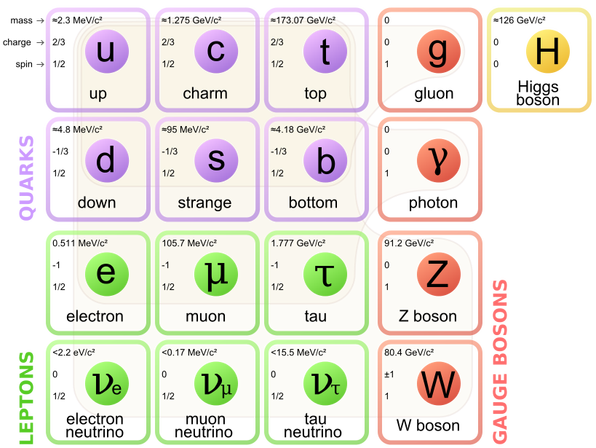
\includegraphics[scale=0.45]{the-standard-model.png}
\caption{Elementary particles of the Standard Model.}
\end{figure}
\\By leaving apart the gravitational interaction, every interaction is known to be mediated by a boson's exchange. The gauge sector is so composed of eight gluons which are the gauge bosons of SU(3)$_{c}$ and the $\gamma$, W$^{\pm}$ and Z$^0$ particles which are the four gauge bosons of \mbox{SU(2)$_{L}$ $\otimes$ U(1)$_{Y}$}. The gluons are massless, electrically neutral and carry color quantum number
\footnote{There are, in fact, eight gluons belonging to an SU(3) octet representation.}. The consequence of the gluons being colorful is that self-interaction terms will appear in the Lagrangian. The weak bosons W$^{\pm}$ and Z$^0$, where W$^{\pm}$ are charged $Q=\pm1$ respectively and Z$^0$ is electrically neutral, are massive and can self-interact as well as the gluons. The photon $\gamma$ is massless, chargeless and not self-interacting\cite{herrero1998standard}.
Actually, both the electromagnetic and the weak interaction are the manifestations at different energy scales of the same, much more fundamental, interaction: the electroweak interaction.

\section{Strong interactions}
The Quantum Chromodynamics (QCD) is the theory underlying the strong interaction. The QCD is a non-Abelian quantum gauge theory, based on the $SU(3)_c$ gauge group, acting on a degree of freedom called 'colour'. At very short wavelenghts it is essencially the theory of the free strongly interacting quarks and gluons, but at longer wavelenghts much more complex partonic bound states emerge, forming the colorless hadrons.
\\
The Lagrangian density describing QCD is 
\begin{equation}
\mathcal{L} = \bar{\psi_q^i}i\gamma^{\mu}(D_{\mu})_{ij}\psi_q^j - m_q\bar{\psi_q^i}\psi_{qi} - \frac{1}{4}F_{\mu\nu}^aF^{\mu\nu,a}
\end{equation}
where $\psi_q^i$ denotes a quark field with colour index i, $\psi_q = (\psi_q^R, \psi_q^G, \psi_q^B)^T$, and the covariant derivative responsible of the interactions is described by
\begin{equation}
(D_{\mu})_{ij} = \delta_{ij}\partial_{\mu} - ig_st_{ij}^aA_{\mu}^a
\end{equation}
The gauge fields $A_{\mu}^a$ coming from $(D_{\mu})_{ij}$ are 8 in total and they represent the eight colorfull gluon fields.
\\
Tipically, color is not present in the final state. Therefore, the fields describing particles will always contain the average over all possible incoming colours and sums over all possible outgoing colours\cite{Skands_2013}.
\\
The modern theory of the strong interactions, compared to its simple structure, shows lots of different features like colour confinement and asymptotic freedom, both due to the peculiar behaviour of the strong coupling constant $\alpha_s$.

\subsection{The running coupling constant in QCD}
The behaviour of the coupling constant is well determined by the evolution of the $\beta$ function, when the renormalization scale M is increased. This function comes from the Callan-Symanzik equation\cite{PhysRevD.2.1541, symanzik1970}
\begin{equation}
\left[ M \frac{\partial}{\partial M} + \beta(\lambda)\frac{\partial}{\partial \lambda} + n \gamma(\eta)\right]G^{(n)}(\{x_i\}; M, \lambda) = 0
\end{equation}
where $G^{(n)}(x_1,\cdots, x_n)$ stands for the \emph{n}-point Green's function and $\beta$ and $\gamma$ are two dimensionless parameters
\begin{equation}
\beta \equiv \frac{M}{\delta M}\delta{\lambda}\:; \hspace{1cm} \gamma \equiv - \frac{M}{\delta M}\delta \eta\:.
\end{equation}
It asserts that there exist two universal functions $\beta(\lambda)$ and $\gamma(\eta)$, related to the shifts of the coupling constant $\lambda$ and field strength $\eta$, that compensate for the shift of the Green's function in the renormalization scale $M$.
\\\\
Going more into details, the evolution of the $\beta$ function, giving the rate at which the renormalized coupling constant changes, determines the strength of the interaction and the conditions under which perturbation theory is valid.
\\
The calculation of Feynman diagrams at higher orders brings along with it some divergences in the matrix element, due to radiative corrections entering in the process. That issue is settled by the addition of some counterterms to subtract the ultraviolet divergences. Since Green's functions depend on $M$ through the counterterms, $\beta$ can be computed from the counterterms arising from the all possible corrections. Thus, at lower order,
\begin{equation}
\beta(g) = gM\frac{\partial}{\partial M}(-\delta_1+\delta_2+\tfrac{1}{2}\delta_3)\:.
\label{beta_function}
\end{equation}
Whether for Abelian quantum gauge theories the first two counterterms cancel each other leaving just the third, for non-Abelian quantum gauge theories, as QCD, all the counterterms get into the calculation with the convention
\\\\
\phantom{i}
\begin{figure*}[h]
\centering
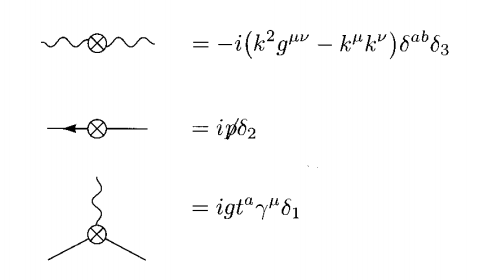
\includegraphics[scale=0.5]{counterterms.png}
\end{figure*}
\phantom{i}
\\\\
In order for the counterterms to cancel the divergences, from the computation of the radiative corrections at first order emerged that
\begin{align}
\begin{split}
\delta_1 &= - \frac{g^2}{(4\pi)^2}\frac{\Gamma(2-\frac{d}{2})}{(M^2)^{2-d/2}}[C_2(r)+C_2(G)] \\
\delta_2 &= - \frac{g^2}{(4\pi)^2}\frac{\Gamma(2-\frac{d}{2})}{(M^2)^{2-d/2}}C_2(r) \\
\delta_3 &= \frac{g^2}{(4\pi)^2}\frac{\Gamma(2-\frac{d}{2})}{(M^2)^{2-d/2}}\Bigl[\frac{5}{3}C_2(G)-\frac{4}{3}n_fC(r)\Bigr]
\end{split}
\label{counterterms}
\end{align}
where $C$ and $C_2$ are coefficients deriving from the group theory\footnote{Given a symmetry group G, the representation matrices in the irreducible rappresentation $r$ are $t_r^a$, generally known as \emph{generators}, which satisfy the commutation relation 
\begin{equation*}
\centering
[t^b;t^c]=if^{bcd}t^d \;.
\end{equation*}
As long as the generators are Hermitian, they satisfy the two relations
\begin{equation*}
tr[t_r^at_r^b] = C(r)\delta^{ab}; \hspace{0.3cm} f^{acd}f^{bcd} = C_2(G)\delta^{ab}
\end{equation*}
where $C_2(G)$ is the \emph{quadratic Casimir operator} of the adjoynt representation of the group.}, $M$ is the renormalization scale and $n_f$ is the fermion's number for the theory.
\\\\
Plugging the three counterterms of Eq.(\ref{counterterms}) into the $\beta$ function (Eq.(\ref{beta_function})), it turns out to be
\begin{equation}
\beta(g) = -\frac{g^3}{(4\pi)^2}\Bigl[\frac{11}{3}C_2(G)-\frac{4}{3}n_fC(r)\Bigr] \;.
\label{beta_function_final}
\end{equation}
In QCD with three colors, described by an $SU(3)$ gauge theory with fermions in the fundamental representation, Eq.(\ref{beta_function_final}) becomes
\begin{equation}
\beta(g) = -\frac{g^3}{(4\pi)^2}\Bigl[11-\frac{2}{3}n_f\Bigr] \;.
\end{equation}
The renormalized coupling constant obtained from the renormalization group equation\footnote{The \emph{renormalization group equation} permits to derive the renormalized coupling constant once computed $\beta$ frunction
\begin{equation*}
\frac{d}{d\mbox{log}(Q/M)}\bar{g} = \beta(\bar{g}) \;.
\end{equation*}} is
\begin{equation}
\alpha_s(Q) = \frac{\alpha_s}{1+(\frac{\alpha_s}{2\pi}[11-\frac{2}{3}n_f]\mbox{log}(k/M))}
\label{alpha_strong}
\end{equation}
It becomes easy to note how for a sufficiently small number $n_f$ of fermions, QCD becomes \emph{asymptotycally free}, because the strong coupling constant in Eq.(\ref{alpha_strong}) tends to zero at large momenta. On the other hand, $\alpha_s$ increase exponentially as momentum transfert decrease, exhibiting the \emph{color confinement} phenomenon \cite{Peskin:1995ev}.
\begin{figure}[t]
\centering
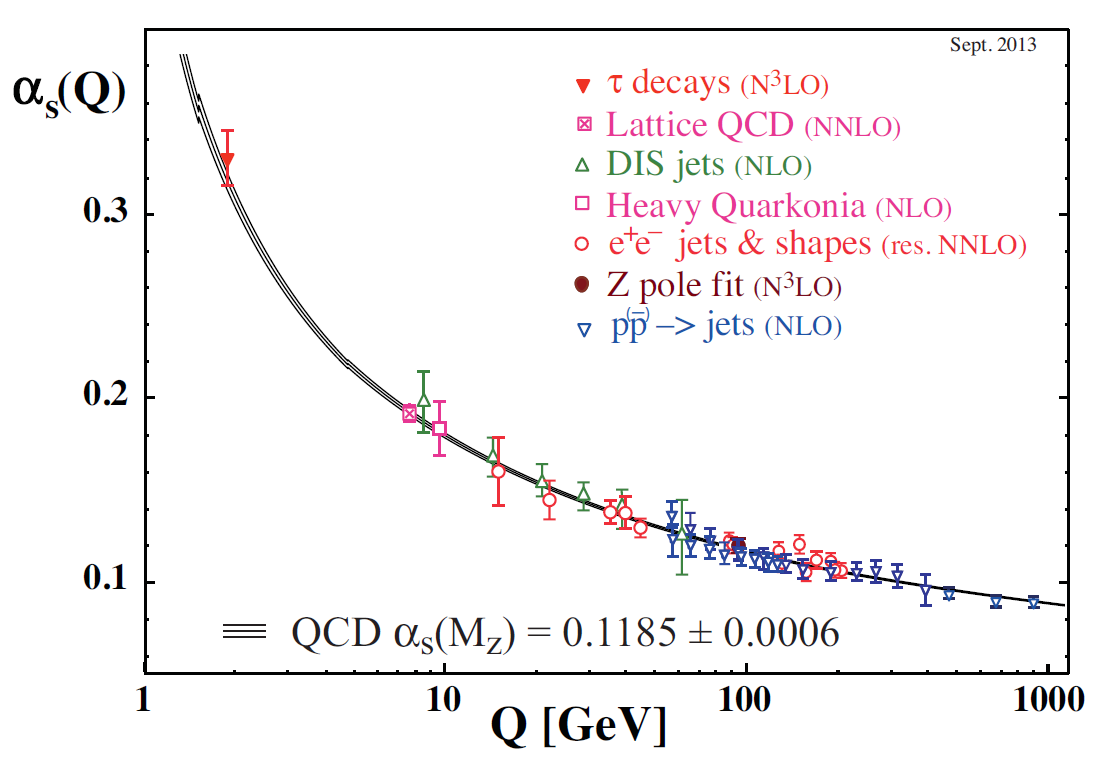
\includegraphics[scale=0.3]{QCD-running-coupling.png}
\caption{The plot shows the behaviour of the strong coupling constant $\alpha_s$, as a function of the transfer momentum $Q$. }
\end{figure}

\subsection{Hard hadronic scattering and the proton structure}
The main difference between leptons and hadrons, making the study of the latter of wide interest, lies in the fact that hadrons are not elementary particles, but have a structure containing colorless combinations of valence quarks plus virtual pairs of quarks/anti-quarks known as \emph{sea quarks}. Sea quarks arise from gluon splitting; a pair of quarks can in turn annihilate producing a gluon. In addition, gluons are present in the sea also owing to the three-gluon and four-gluon vertices.
\\
Colliding hadrons, protons more precisely, becomes a quite hard process to describe as energy is increased. After a certain threshold, in fact, the proton breaks up, manifesting his complex internal structure and making the scattering of the constituent quarks and gluons possible, such as $qq$, $q\bar{q}$, $gq$, $g\bar{q}$, $gg$.
\\
In proton collisions, being the elementary interaction at parton level, each of the scattering constituents carries a different fraction \emph{x} of the proton four-momentum, known as Bjorken's scaling variable \cite{altarelli2013collider}. The rescaled center-of-mass energy, taking into consideration the fraction \emph{x} of both partons, turns out to be $\sqrt{\hat{s}}=\sqrt{x_1x_2s}$, where $s$ is the center-of-mass energy of the incoming protons and $x_1$ and $x_2$ represent the fraction of the momentum carried by each of the interacting partons. With this interpretation, the cross section describing a typical $pp \rightarrow X$ process has to include a term that describes the partonic hard scattering, calculated using perturbative Quantum Field Theory, and factors for the incoming flux of partons, the \emph{parton distribution functions} (PDF).
\\
Considering that, the cross section for a typical $pp$ collision takes the form
\begin{equation}
\sigma(pp \rightarrow X) = \displaystyle\sum_{i,j} \int dx_1 \int dx_2f_i(x_1,\mu_F^2)f_j(x_2,\mu_F^2)\cdot\hat{\sigma}_{ij \rightarrow X}(x_1x_2s,\mu_R^2, \mu_F^2)
\label{pp_cross_section}
\end{equation}
In Eq.(\ref{pp_cross_section}) the sum runs over all possible initial-state partons, with longitudinal momentum $x_{1,2}$, that can give rise to a final state $X$ at a center-of-mass energy of $\sqrt{x_1x_2s}$ \cite{Butterworth_2012}. The \emph{factorization scale} parameter $\mu_F$ represent the scale at which the separation between the hard perturbative interaction and the long distance non-perturbative evolution of the produced partons occurs.The $\hat{\sigma}_{i,j \rightarrow X}$ term describes the elementary partonic cross section at the scale $\mu_F$ and $\mu_R$, where $\mu_R$ is the \emph{renormalization scale}, introduced in perturbative QCD to cut ultraviolet divergences. The two terms $f_i(x_1,\mu_F^2)$ and $f_j(x_2,\mu_F^2)$ are the PDFs of each parton involved into the process and describe the probability density for a parton to be found within the incoming pronton and to carry a certain fraction of its momentum.
\\
Since QCD doesn't predict the parton content of the proton, the shapes of the PDFs are obtained by a fit to data at different scales $Q^2$ in various processes, using the DGLAP evolution equations \cite{ALTARELLI1977298}. Introducing the variable $\tau = \ln(Q^2/\mu^2)$ and denoting the gluon distribution function in the nucleon by $g(x,\tau)$ and that of the quark by $q(x,\tau)$, the formula to derive the quark distribution functions, including the gluon splitting effect too, can be written as \cite{nagashima2010elementary}
\begin{equation}
\frac{dq(x,\tau)}{d\tau} = \frac{\alpha_s}{2\pi}\int_x^1\frac{dy}{y}\Bigl[q(y,\tau)P_{q\leftarrow q}\Bigl(\frac{x}{y}\Bigr)+g(y,\tau)P_{q\leftarrow g}\Bigl(\frac{x}{y}\Bigr)\Bigr]
\end{equation}
where $P_{a\leftarrow b}$ are the splitting functions for the parton $a$ to emit the parton $b$.
\\ 
Similarly, the gluon distribution function can be derived using
\begin{equation}
\frac{dg(x,\tau)}{d\tau} = \frac{\alpha_s}{2\pi}\int_x^1\frac{dy}{y}\Bigl[q(y,\tau)P_{g\leftarrow q}\Bigl(\frac{x}{y}\Bigr)+g(y,\tau)P_{g\leftarrow g}\Bigl(\frac{x}{y}\Bigr)\Bigr]
\end{equation}
These kind of equations permit to determine the behavior of the flux of gluons and quarks within the proton in terms of PDFs at all values of $Q^2$, above the input scale $Q_0^2$ at which they are parametrized as a function of $x$.
\\
In Figure \ref{pdf} you can see how, for big momentum fractions (large $x$-values) the main contributions come from $u$ and $d$ quarks, with about a 2:1 ratio, while other flavours are virtually absent
\footnote{In this way, we can consider the proton made of two $up$-quarks and one $down$-quark.}.
With momentum decreasing, the contribution of the other flavours different from $u$ and $d$, generated from the $g \rightarrow qq$ splitting starts also to increase.
\\
At low energies the main contribution to the parton flux comes from the gluons
\footnote{Notice how in Figure \ref{pdf} the gluons distribution is scaled down by a $1/10$ factor, so its contribution is extremely high compared to the one coming from the various quarks.}
and this feature is further accentuated by increasing the $Q^2$ scale.
\begin{figure}[t]
\centering
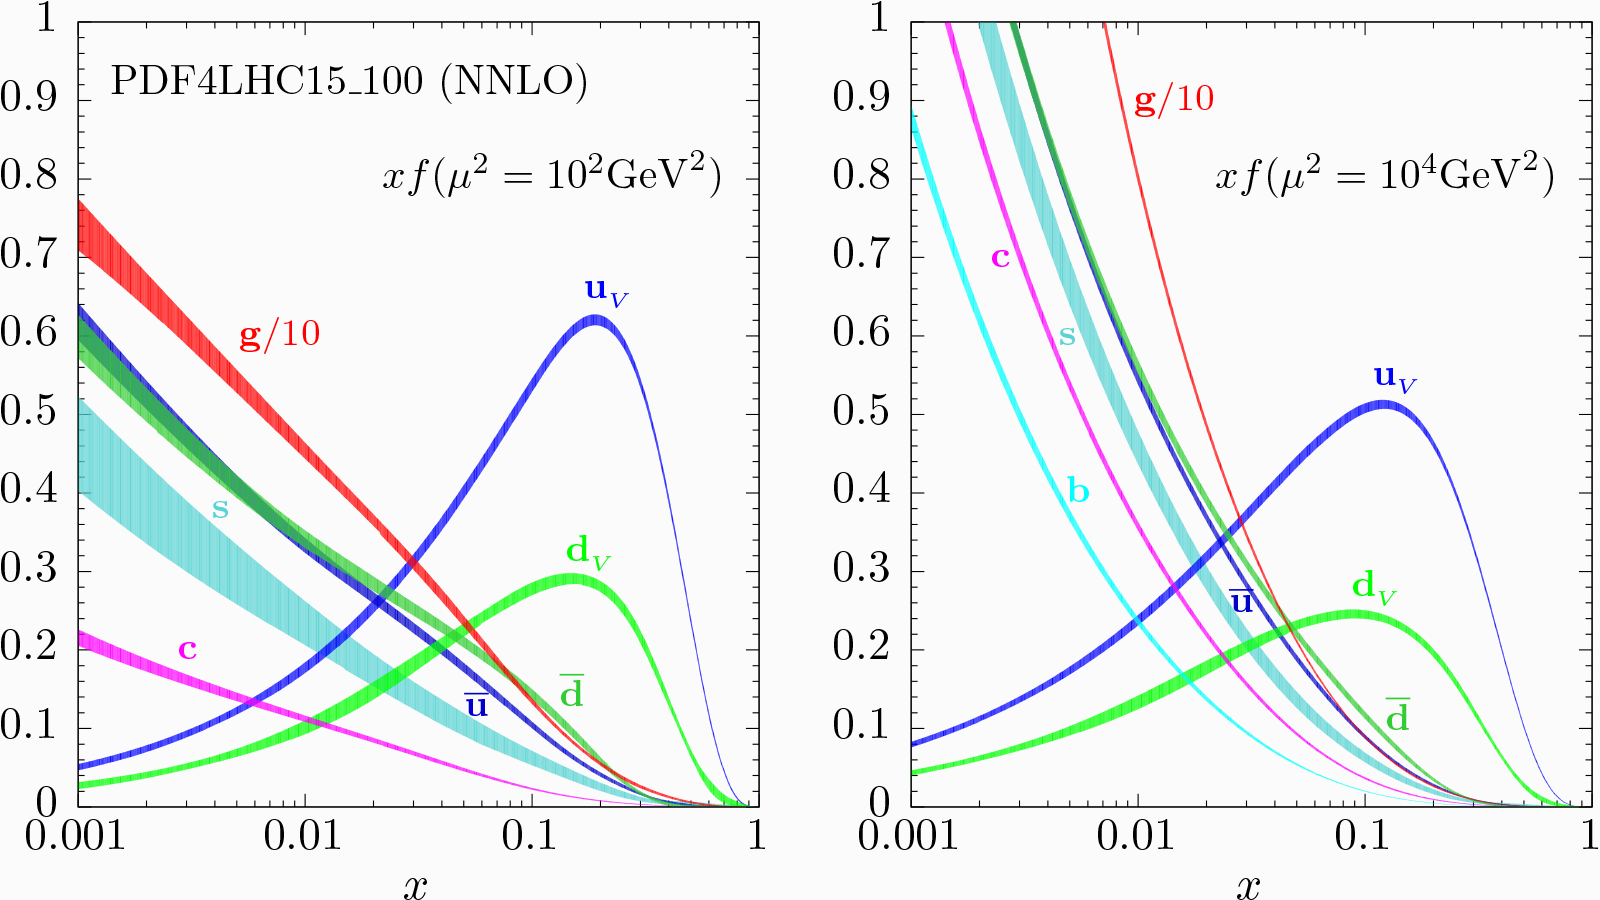
\includegraphics[scale=0.22]{pdf.png}
\caption{PDF's $x$ dependencies on a logarithmic scale for two different energy scales. On the left a "low" scale, while on the the right an "high" scale, typical from LHC, are presented. }
\label{pdf}
\end{figure}

\section{Electroweak interactions}
\emph{<<Leptons interact only with photons and with the intermediate bosons that presumably mediate weak interactions. What could be more natural than to unite these spin-one bosons
into a multiplet of gauge fields?>>} (S. Weinberg, 1967)\cite{PhysRevLett.19.1264}.
\\\\
The electroweak theory is an \mbox{SU(2)$_L$ $\otimes$ U(1)$_Y$} local gauge theory, where SU(2)$_L$ group only left-handed particles and refers to the weak isospin charge $I$, while U(1)$_Y$ is related to the weak hypercharge $Y$, both connected together by the equation:
\begin{equation}
Y = 2(Q-I_3)
\end{equation}
Due to the nature of the theory, its Lagrangian needs to be invariant under \mbox{SU(2) $\otimes$ U(1)} global gauge transformations.
The electroweak Lagrangian which involve only gauge bosons, fermions and their interactions turns out to be
\begin{align}
\begin{split}
\mathcal{L} = - \frac{1}{4} \displaystyle\sum_{A=1}^3F_{\mu\nu}^AF^{A\mu\nu} - \frac{1}{4} B_{\mu\nu}&B^{\mu\nu} + \\ 
 + \bar{\psi}_Li&\gamma^{\mu}D_{\mu}\psi_L + \bar{\psi}_Ri\gamma^{\mu}D_{\mu}\psi_R
 \end{split}
\label{EW_lagrangian}
\end{align}
where the gauge fields $B_{\mu\nu}$ and $F_{\mu\nu}^A$ are
\begin{align}
\begin{split}
&B_{\mu\nu} = \partial_{\mu}B_{\nu} - \partial_{\nu}B_{\mu} \\
&F_{\mu\nu}^A = \partial_{\mu}W_{\nu}^A - \partial_{\nu}W_{\mu}^A - g\epsilon_{ABC}W_{\mu}^BW_{\nu}^C
\end{split}
\end{align}
and $D_{\mu}$ is the covariant derivatives for the gauge group, usefull to introduce the interactions in the Lagrangian (\ref{EW_lagrangian}) and making it invariant under local gauge transformations:
\begin{equation}
D^{\mu} = \partial^{\mu} + ig \boldsymbol{\tau} \cdot \hat{\boldsymbol{W}}^{\mu} /2+ig'\hat{B}^{\mu} /2
\end{equation}
where $\boldsymbol{\tau} = (\tau_1, \tau_2, \tau_3)$ are the Pauli matrices and $\hat{\boldsymbol{W}}^{\mu} = (\hat{W}_1^{\mu}, \hat{W}_2^{\mu}, \hat{W}_3^{\mu})$ stands for the three generators of the SU(2)$_L$ group. 
\\
The four gauge fields coming from the generators of the group cannot be considered as the physical electroweak gauge bosons, because of the mass issue: the four gauge fields are all massless, while in the physical ones the three weak bosons $W^{\pm}$ and $Z^0$ are actually massive
\footnote{($m_W = 80.370 \pm 0.019$ GeV, $m_Z = 91.187 \pm 0.007$ GeV) \cite{Aaboud_2018, Arnaudon}}\cite{altarelli2000standard}.
The physical bosons come up from the symmetry-breaking mechanism, discussed further below, through a mixing between the unphysical fields
\begin{align}
\begin{split}
&W_{\mu}^{(\pm)} = \frac{1}{\sqrt{2}}(W_{\mu}^1 \pm iW_{\mu}^2) \\
&Z_{\mu}^0 = cos\theta_W W_{\mu}^3 + sin\theta_W B_{\mu} \\
&A_{\mu} = -sin\theta_W W_{\mu}^3 + cos\theta_W B_{\mu} 
\end{split}
\label{EWbosons}
\end{align}
The fields in (\ref{EWbosons}) are in fact the physical particle fields, where $W_{\mu}^{\pm}$ stand for the electrically charged weak interacting bosons, $Z_{\mu}^0$ represents the electrically neutral weak interacting boson and $A_{\mu}$ denote the photon, the only field left massless after the symmetry-breaking process\cite{Weinberg:1996kr}.
\\ \\
The Feynman rules of the theory show several vertices between bosons and fermions, in addition to some self-interacting vertices between the gauge bosons, due to the non-Abelianity of \mbox{$SU(2)_L \otimes U(1)_Y$}.

\begin{figure}[h]
\centering
\subfloat{\feynmandiagram [small, horizontal=e to f] {
  e -- [boson, edge label = \small$\gamma$, near start]  f,
  h [particle =$f$] -- [fermion] f -- [fermion] i[particle=$f$],
};} \hspace{0.5cm}
\subfloat{\feynmandiagram [small, horizontal=e to f] {
  e -- [boson, edge label = \small$W$, near start]  f,
  h [particle =$\nu_l$] -- [fermion] f -- [fermion] i[particle=$l$],
};} \hspace{0.5cm}
\subfloat{\feynmandiagram [small, horizontal=e to f] {
  e -- [boson, edge label = \small$W$, near start]  f,
  h [particle =$q_i$] -- [fermion] f -- [fermion] i[particle=$q_j$],
};} \hspace{0.5cm}
\subfloat{\feynmandiagram [small, horizontal=e to f] {
  e -- [boson, edge label = \small$Z$, near start]  f,
  h [particle =$f$] -- [fermion] f -- [fermion] i[particle=$f$],
};} \\ \vspace{0.5cm}
\subfloat{\feynmandiagram [small, horizontal=e to f] {
  e -- [boson, edge label = \small$\gamma/Z$, near start]  f,
  h -- [boson, edge label=\small$W$, near start] f -- [boson, edge label=$\small{W}$, near end] i,
};} \hspace{0.5cm}
\subfloat{\feynmandiagram [small, horizontal=i1 to f2] {
  i1 -- [boson, edge label=\small$W$, near start] c -- [boson, edge label=\small$W$, near end] f1,
  i2 -- [boson, edge label=\small$W$, near start] c -- [boson, edge label=\small$W$, near end] f2,
};}\hspace{0.5cm}
\subfloat{\feynmandiagram [small, horizontal=i1 to f2] {
  i1 -- [boson, edge label=\small$W$, near start] c -- [boson, edge label=\small$\gamma/Z$, near end] f1,
  i2 -- [boson, edge label=\small$\gamma/Z$, near start] c -- [boson, edge label=\small$W$, near end] f2,
};}\\\hspace{0.3cm}
\caption{The Feynman vertices for the electroweak interaction. On the top the fermions couplings are displayed, while on the bottom the self-interacting couplings are shown.}
\end{figure}

\subsection{The Higgs Field and the Mechanism}
The \emph{Higgs mechanism} is essential to explain how gauge vector bosons acquire mass through a spontaneous symmetry breaking
\footnote{The \emph{spontaneous symmetry breaking} describes systems where the lowest energy vacuum solutions do not exhibit the same symmetry of the Lagrangian. In these vacuum solutions, the symmetry is broken for perturbations around them even though the entire Lagrangian retains that symmetry.}
. Without this mechanism, in fact, all bosons would be considered massless and this doesn't reflect the experimental evidences. 
\\\\
The main difference between a vector massive field and a massless one lies in the number of degrees of freedom, three in the former case, two in the latter in particular. This discrepancy indicates that some additional fields must be present in order to give mass to the originally massless gauge bosons.
\\\\
The fundamental idea presented by Higgs is to assume that a "hidden" field has to exists, whose potential's ground state, shown in Figure \ref{mexican_hat}, breaks the Lagrangian symmetry spontaneously \cite{Aitchison_Hey}.
\\
That field, known as the \emph{Higgs field}, permeates every region of the Universe. At temperatures high enough, all particles are massless and the symmetry is unbroken. Once a critical temperature is reached, typically shortly after the hot big bang, the Higgs field develops a vacuum expectation value (VEV) different from $0$
\footnote{The \emph{vacuum expectation value} of a field is the lowest-energy configuration that satisfies the classical equations of motion \cite{Schwartz:2013pla}.} and so the symmetry breaks up, giving masses to the particles, both bosons and fermions, through the Higgs boson interactions.
\begin{figure}[t]
\centering
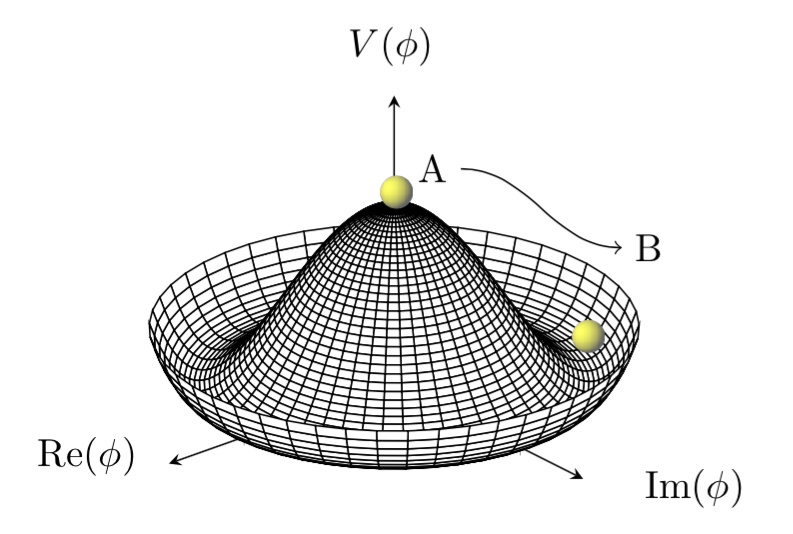
\includegraphics[scale=0.36]{higgs_potential.png}
\caption{Graphical representation of the Higgs potential $V(\phi)$, usually known as "mexican hat" potential. The point A is the high energy symmetric local maximum, while the point B is the low energy asymmetric local minimum. The symmetry breaks up once a particle flows from A to B, choosing a particular local minimum among the continuum set of low energy minima.}
\label{mexican_hat}
\end{figure}
The geometric structure of the Higgs field is an $SU(2)$ doublet, which is a scalar under Lorentz transformations, and under $U(1)$ rotations, it is multiplied by a phase.
\\
The four degrees of freedom so introduced are the real actors of the mass generation: three out of four of them mix with the originally massless vector bosons and the only single remaining degree of freedom becomes the new scalar Higgs boson.
\\\\
From the quantitative point of view, the simplest choice for a field with at least the three necessary degrees of freedom for the success of the mechanism is a complex $SU(2)$ doublet of scalar fields $\hat{\phi}$
\begin{equation}
\hat{\phi} = \begin{pmatrix}
\hat{\phi}^+ \\ \hat{\phi}^0 
\end{pmatrix} \text{,} \hspace{0.4cm} Y_{\phi}=+1
\end{equation}
described by the Lagrangian
\begin{equation}
\hat{\mathcal{L}}_{\phi} = (\partial_{\mu}\hat{\phi}^\dag)(\partial^{\mu}\hat{\phi})+\mu^2\hat{\phi}^\dag\hat{\phi}-\frac{\lambda}{4}(\hat{\phi}^\dag\hat{\phi})^2
\label{Higgs_lagrangian}
\end{equation}
This Lagrangian is invariant under $SU(2)$ and $U(1)$ global transformations. To make it invariant under local transformations too, you need to introduce three gauge fields for the $SU(2)$ group ($\hat{W}_i^{\mu}(x)$ with $i=1,2,3$) and the $\hat{B}^{\mu}(x)$ field for the group $U(1)$. 
\\
These additions can be inserted by the use of the covariant derivative
\begin{equation}
\hat{D}^{\mu} \hat{\phi} = (\partial^{\mu} + ig \boldsymbol{\tau} \cdot \hat{\boldsymbol{W}}^{\mu} /2+ig'\hat{B}^{\mu} /2)\hat{\phi}
\end{equation}
where $\boldsymbol{\tau} = (\tau_1, \tau_2, \tau_3)$ is the three Pauli matrices set.
\\\\
The Lagrangian for the Higgs sector consisting of the gauge fields and the Higgs fields (without gauge-fixing ang ghost terms) so becomes
\begin{align}
\hat{\mathcal{L}}_{G\phi} = &(\hat{D}_{\mu}\hat{\phi})^{\dag}(\hat{D}^{\mu}\hat{\phi})+\mu^2\hat{\phi}^{\dag}\hat{\phi}-\frac{\lambda}{4}(\hat{\phi}^{\dag}\hat{\phi})^2 \\
&-\frac{1}{4}\hat{\boldsymbol{F}}_{\mu\nu}\cdot\hat{\boldsymbol{F}}^{\mu\nu}-\frac{1}{4}\hat{G}_{\mu\nu}\hat{G}^{\mu\nu}
\label{Higgs_local_invariant}
\end{align}
where $\hat{\boldsymbol{F}}_{\mu\nu}$ is the $SU(2)$ field strength tensor for the gauge fields $\hat{\boldsymbol{W}}^{\mu}$ and $\hat{G}_{\mu\nu}$ is the $U(1)$ field strength tensor for the gauge field $\hat{B}^{\mu}$ respectively given by
\begin{align}
\hat{\boldsymbol{F}}^{\mu\nu}& \hspace{0.1cm}=\hspace{0.1cm} \partial^{\mu}\hat{\boldsymbol{W}}^{\nu}-\partial^{\nu}\hat{\boldsymbol{W}}^{\mu}-g\hat{\boldsymbol{W}}^{\mu}\times\hat{\boldsymbol{W}}^{\nu} \\
\hat{G}^{\mu\nu}& \hspace{0.1cm}=\hspace{0.1cm} \partial^{\mu}\hat{B}^{\nu}-\partial^{\nu}\hat{B}^{\mu}
\end{align}
The plus sign in the $\mu^2$ term in the Eq.(\ref{Higgs_lagrangian}) and in Eq.(\ref{Higgs_local_invariant}) reflects the symmetry breaking. That particular choice for the sign creates the typical shape visible in Figure \ref{mexican_hat}, and allows the field $\phi(x)$ to acquire a vacuum expectation value at the minimum of the potential
\begin{equation}
\langle\phi\rangle_0 \equiv \langle0|\phi|0\rangle = \begin{pmatrix} 
		0 \\ 
		\frac{v}{\sqrt{2}} 
		\end{pmatrix} \hspace{0.4cm} \text{with} \hspace{0.4cm} v = \Bigl(-\frac{\mu^2}{\lambda}\Bigr)^{1/2}
\label{vev}
\end{equation}
It's now time to apply perturbation theory, expanding around one of the minima $v$ by defining the physical Higgs field $\hat{H}$ and parametrizing $\hat{\phi}$ as
\begin{equation}
\hat{\phi} = \begin{pmatrix} 
		0 \\ 
		\frac{1}{\sqrt{2}}(v+\hat{H}) 
		\end{pmatrix}
\label{expansion}
\end{equation}
Inserting Eq.(\ref{expansion}) in the local gauge invariant Lagrangian and making the symmetry breaking manifest, the free fields quadratic parts of Eq.(\ref{Higgs_local_invariant}) can be written as
\begin{align}
\begin{split}
\hat{\mathcal{L}}^{free}_{G\phi} \hspace{0.2cm} =& \hspace{0.4cm} \frac{1}{2}\partial_{\mu}\hat{H}\partial^{\mu}\hat{H}-\mu^2\hat{H}^2 \\
& -\frac{1}{4}(\partial_{\mu}\hat{W}_{1\nu}-\partial_{\nu}\hat{W}_{1\mu})(\partial^{\mu}\hat{W}_1^{\nu}-\partial^{\nu}\hat{W}_1^{\mu}) + \frac{1}{8}g^2v^2\hat{W}_{1\mu}\hat{W}_1^{\mu} \\
& -\frac{1}{4}(\partial_{\mu}\hat{W}_{2\nu}-\partial_{\nu}\hat{W}_{2\mu})(\partial^{\mu}\hat{W}_2^{\nu}-\partial^{\nu}\hat{W}_2^{\mu}) + \frac{1}{8}g^2v^2\hat{W}_{2\mu}\hat{W}_2^{\mu} \\
& -\frac{1}{4}(\partial_{\mu}\hat{Z}_{\nu}-\partial_{\nu}\hat{Z}_{\mu})(\partial^{\mu}\hat{Z}^{\nu}-\partial^{\nu}\hat{Z}^{\mu}) + \frac{1}{8}g^2v^2\hat{Z}_{\mu}\hat{Z}^{\mu} \\
& -\frac{1}{4}\hat{F}_{\mu\nu}\hat{F}^{\mu\nu}
\end{split}
\label{expanded_lagrangian}
\end{align}
in unitary gauge
\footnote{The \emph{unitary gauge} or unitarity gauge is a particular choice of a gauge fixing in a gauge theory with a spontaneous symmetry breaking. In this gauge, the scalar field $\phi$ responsible for the Higgs mechanism are transformed into a basis in which their Goldstone boson components are set to zero. Writing the field $\phi$ in terms of four fields $\hat{\theta}_{1,2,3}(x)$ and $H(x)$, the unitary gauge allows to rewrite it as
\footnotesize
\begin{equation*}
\hat{\phi} = \begin{pmatrix} 
		\hat{\theta_2} + i\hat{\theta_1} \\ 
		\frac{1}{\sqrt{2}}(v+\hat{H}) - i\hat{\theta_3} 
		\end{pmatrix}
		= \exp^{i\theta_a(x)\tau^a(x)/v}\begin{pmatrix} 
		0 \\ 
		\frac{1}{\sqrt{2}}(v+\hat{H}) 
		\end{pmatrix}
\end{equation*}
making the manifest number of scalar degrees of freedom minimal.}
, where
\begin{align}
\hat{F}^{\mu\nu} =& \hspace{0.1cm} \partial^{\mu}\hat{A}^{\nu} - \partial^{\nu}\hat{A}^{\mu} \\
\hat{Z}^{\mu} =& \hspace{0.1cm} \cos{\theta}_W\hat{W}_3^{\mu} - \sin{\theta}_W\hat{B}^{\mu} \\
\hat{A}^{\mu} =& \hspace{0.1cm} \sin{\theta}_W\hat{W}_3^{\mu} + \cos{\theta}_W\hat{B}^{\mu}
\end{align}
with
\begin{equation}
\cos{\theta}_W = \frac{g}{\sqrt{g^2+g'^2}} \hspace{0.2cm} \text{,} \hspace{0.4cm} \sin{\theta}_W = \frac{g'}{\sqrt{g^2+g'^2}}
\end{equation}
In Eq.(\ref{expanded_lagrangian}) it's easy to see how, after the spontaneous symmetry breaking due to the vacuum expectation value, the mass terms for the physical gauge bosons appear as well as for the Higgs boson itself
\footnote{Both charged weak interacting bosons $W$s have the same mass term, while the only field left massless after the symmetry breaking remains the photon field, as it should be.}.
From terms which are bilinear in the fields $\hat{W}_1^{\mu}$, $\hat{W}_2^{\mu}$, $\hat{Z}^{\mu}$ you can derive the explicit form for the masses of the particles
\begin{equation}
m_H = \sqrt{2} \mu = \frac{\sqrt{\lambda}v}{\sqrt{2}} \text{,} \hspace{0.4cm} m_W = \frac{gv}{2} \text{,} \hspace{0.4cm} m_Z = \frac{m_W}{\cos{\theta}_W} 
\end{equation}
In a similar way as the one seen for bosons, also for the fermionic sector of the Higgs interaction Lagrangian is possible to give mass to fermions, without introducing an explicit mass term in the Lagrangian. Using electrons as an example, it could be assumed an hypothetical coupling between an electron-type SU(2) doublet
\begin{equation}
\begin{pmatrix}
\nu_{e} \\ e^- 
\end{pmatrix}_L \hspace{0.2cm} \text{,}
\end{equation}
the Higgs doublet $\phi$ and the R-component of the electron field preserving the SU(2)$_L$ invariance, feature required by the electroweak interaction nature. The Lagrangian for these kinds of couplings, usually known as \emph{Yukawa couplings}, can be written as 
\begin{equation}
\mathcal{\hat{L}}_{\text{int}} = \lambda_e\Bigl(\bar{\hat{l}}_{eL}\hat{\phi} \hat{e}^-_R + \hat{\phi}^{\dag}\hat{e}^-_R\hat{l}_{eL}\Bigr)
\label{lepton_lagrangian}
\end{equation}
where $\lambda_e$ is the self-coupling of the fermion, an electron in this case and it is an arbitrary parameter of the theory.Expanding the Lagrangian (\ref{lepton_lagrangian}) around a minimum of the Higgs field, it turns out to be
\begin{align}
\begin{split}
\mathcal{\hat{L}}_{\text{Yukawa}} =& \frac{\lambda_ev}{\sqrt{2}}\Bigl(\bar{\hat{e}}^-_L\hat{e}^-_R + \bar{\hat{e}}^-_R\hat{e}^-_L\Bigr) + \frac{\lambda_e}{\sqrt{2}}\Bigl(\bar{\hat{e}}^-_L\hat{e}^-_R + \bar{\hat{e}}^-_R\hat{e}^-_L\Bigr)\hat{H} \\
=& m_e\bar{\hat{e}}\hat{e} + \frac{m_e}{v}\bar{\hat{e}}\hat{e}\hat{H} \hspace{0.4cm} \text{.}
\end{split}
\label{lepton_expanded}
\end{align}
The first term of the Lagrangian (\ref{lepton_expanded}) is exactly the Dirac mass term for the electron, making easy to recognise
\begin{equation}
m_e = \lambda_ev/\sqrt{2}
\end{equation}
It seeks to identify the last term of the Lagrangian (\ref{lepton_expanded}) as a coupling between the electron Higgs fields, implying also no neutrino-Higgs interactions, due to the absence of $\nu_R$ component for the neutrinos field.
\\\\
It is possible to repete this mass generation mechanism for each fermion in the theory and so derive the values for the different masses, as functions of the arbitrary self-coupling of the selected fermion
\begin{equation}
m_f = \lambda_fv/\sqrt{2} \hspace{0.4cm} \text{.}
\end{equation}
In this way the masses are included in the Standard Model, but they are not predicted, thus they must be measured.
\\\\
The Higgs boson interacts with fermions with a strength proportional to their mass $m_f$, therefore it couples more strongly to the heaviest fermions.
\\
Notice how, with the same isodoublet $\hat{\phi}$ of scalar fields, the Higgs mechanism allows to generate the masses for fermions and weak interacting vector bosons $W^\pm$, $Z^0$ leaving massless the photon field, while preserving the \mbox{$SU(2) \times U(1)$} gauge symmetry, which is now hidden by the spontaneous symmetry breaking \cite{Aitchison_Hey, Djouadi_2008}.

\subsection{Higgs boson in the Standard Model}
The massive particle arising from the spontaneously symmetry breaking, known as the \emph{Higgs boson}\cite{PhysRevLett.13.321, PhysRevLett.13.508}, is well described in the first line of Eq.(\ref{expanded_lagrangian}) Lagrangian. The kinetic term, $\frac{1}{2}\partial_{\mu}\hat{H}\partial^{\mu}\hat{H}-\mu^2\hat{H}^2$, comes from the term involving the covariant derivative $|D_{\mu}\phi|^2$, while the mass term derives from the structure of the Higgs potential.
\\
After the vacuum expansion, the terms concerning the mass and the intercations for the Higgs boson in the Lagrangian are
\begin{equation}
\hat{\mathcal{L}}^{int}_{G\phi} \hspace{0.2cm} = \hspace{0.2cm} -\lambda v^2\hat{H}^2 -\lambda v\hat{H}^3 -\frac{\lambda}{2!}\hat{H}^4 
\label{interactions}
\end{equation}
From Eq.(\ref{interactions}) you can see how the particle's mass turns out to be simply as 
\begin{equation}
M_H^2 = 2\lambda v^2 = -2\mu^2
\end{equation}
and the Feynman rules for the Higgs self-interaction vertices (Figure \ref{self_H}) are given by
\begin{equation}
g_{H^3} = (3!)i\lambda v = 3i\frac{M_H^2}{v} \hspace{0.2cm} \text{,} \hspace{0.4cm} g_{H^4} = (4!)i\frac{\lambda}{4} = 3i\frac{M_H^2}{v^2}
\end{equation}
The interaction with gauge bosons and fermions are described by the Higgs boson couplings
\begin{equation}
g_{Hff} = i\frac{m_f}{v} \hspace{0.2cm} \text{,} \hspace{0.4cm} g_{HVV} = -2i\frac{M_V^2}{v} \hspace{0.2cm} \text{,} \hspace{0.4cm} g_{HHVV} = -2i\frac{M_V^2}{v^2}
\end{equation}
The vacuum expectation value for the Higgs field, seen in Eq.(\ref{vev}), is fixed in terms of the $W$ boson mass $M_W$
\begin{equation}
M_W = \frac{1}{2}gv \hspace{0.2cm} \Rightarrow \hspace{0.2cm} v = \frac{2M_W}{g} \simeq \text{246 GeV}
\end{equation}
\begin{figure}[h]
\centering
\subfloat[][]{\feynmandiagram [horizontal=e to f] {
  e -- [scalar, edge label = \small$H$, near start]  f,
  h -- [scalar, edge label = \small$H$, near start] f -- [scalar, edge label = \small$H$, near end] i,
};} \hspace{0.8cm}
\subfloat[][]{\feynmandiagram [horizontal=i1 to f2] {
  i1 -- [scalar, edge label=\small$H$, near start] c -- [scalar, edge label=\small$H$, near end] f1,
  i2 -- [scalar, edge label=\small$H$, near start] c -- [scalar, edge label=\small$H$, near end] f2,
};}
\caption{a)Three-line Higgs self-interacting vertex, b)Four-line Higgs self-interacting vertex.}
\label{self_H}
\end{figure}

\section{The Higgs sector at LHC}
\emph{<<This summer I have discovered something totally useless.>>} (P. W. Higgs, 1964)
\\ \\
In this section the Higgs boson sector will be presented. Starting from the various production modes, it continue with the different decay channels, focusing on $H \rightarrow \gamma \gamma$, which is the channel investigated in this work.
\subsection{Higgs boson production modes}
Being the LHC a proton-proton collider, the main process contributing to the Higgs boson production must contain gluons deriving from the colliding protons.
In order of decreasing cross section, the channels involved into the Higgs production are:
\begin{itemize}
\item \emph{Gluon fusion} (ggH): the most common production mode at LHC over the whole mass spectrum, due to the proton structure. It leads to about 85\% of the total cross section in the mass range of 120-130 GeV. This kind of process requires the fusion of two gluons, producing the Higgs boson through a heavy quark loop, tipically a top quark, because of its heavy mass.
\begin{figure}[H]
\centering
\feynmandiagram [small, horizontal=g1 to t1] {
  g1 --[gluon, edge label=\small$g$] t1 -- [fermion] t2 --[fermion] t3 --[fermion] t1,
  g2 --[gluon, edge label=\small$g$] t2,
  t3 -- [scalar, edge label = \small$H$]  h,
  g1 --[opacity=0] g2,
};
\end{figure}
\item \emph{Vector Boson Fusion} (VBF): this production mode is the second most dominant in the Higgs sector and is the responsible of around 7\% of the total number of Higgs produced in the selected mass range. It consists in the scattering of two incoming quarks, each of them emitting a $W^{\pm}$ or $Z^0$ boson which, in turn, interact to produce the Higgs boson. The peculiar signature of this production is the presence of two high-energy forward jets, arising from the scattered valence quarks of the two protons.
\begin{figure*}[h]
\centering
\begin{tikzpicture}
  \begin{feynman} [small]
  	\vertex (i1);
  	\vertex[right=1.3cm of i1] (v1);
  	\vertex[above right=1.5cm of v1] (f1);
  	\vertex[below right=of v1] (v2);
  	\vertex[right=of v2] (h);
  	\vertex[below left=of v2] (v3);
  	\vertex[left=1.3cm of v3] (i2);
  	\vertex[below right=1.5cm of v3] (f2);
  	
  	\diagram* {
  		(i1) -- [plain, fermion] (v1) -- [plain, fermion] (f1),
  		(i2) -- [plain, fermion] (v3) -- [plain, fermion] (f2),
  		(v1) -- [boson] (v2),
  		(v3) -- [boson, edge label=\small $W/Z$] (v2),
  		(v2) --[scalar, edge label = \small $H$] (h),
  		};
  	\end{feynman}
\end{tikzpicture}
\end{figure*}
\item \emph{Higgsstrahlung} (VH): even if the cross section for this production mode is comparable with the VBF cross section for masses between 120 and 130 GeV. The Higgs boson is emitted with an associated vector boson from a $W^{\pm}$ or $Z^0$ arising from two incoming quarks.
\begin{figure*}[h]
\centering
\feynmandiagram [small, horizontal=a to b] {
i1 -- [fermion] a -- [fermion] i2,
a -- [boson, edge label=\small$W/Z$] b,
f1 -- [boson] b -- [scalar, edge label= \small $H$] f2,
};
\end{figure*}
\item \emph{Top quark associated production} ($t\bar{t}H$): this particular production mode derive from two gluon splitting into two pairs of t-quarks. Just after it, two out of the four produced quarks interact emitting a Higgs boson, while the other two t-quarks will decay\footnote{The t-quark is the only quark which decays instead of hadronize. Because of its huge mass, the t-quark has an extremely short lifetime, predicted in $5 \times 10^{-25} \text{s}$. In this short amount of time the hadronisation process cannot take place and the t-quark decays as a "bare" quark.}
\begin{figure*}[!h]
\centering
\begin{tikzpicture}
  \begin{feynman} [small]
  	\vertex (i1);
  	\vertex[right=1.3cm of i1] (v1);
  	\vertex[above right=1.5cm of v1] (f1);
  	\vertex[below right=of v1] (v2);
  	\vertex[right=of v2] (h);
  	\vertex[below left=of v2] (v3);
  	\vertex[left=1.3cm of v3] (i2);
  	\vertex[below right=1.5cm of v3] (f2);
  	
  	\diagram* {
  		(i1) -- [gluon] (v1) -- [fermion, edge label = \small $t$] (f1),
  		(i2) -- [gluon] (v3)
  		(f2) -- [fermion, edge label = \small $\bar{t}$] (v3),
  		(v1) -- [fermion] (v2),
  		(v3) -- [fermion] (v2),
  		(v2) --[scalar, edge label = \small $H$] (h),
  		};
  	\end{feynman}
\end{tikzpicture}
\end{figure*}
\end{itemize}
The cross sections for all of these processes vary as the mass runs on its energy spectrum. Typically, the production cross sections decrease with the increasing of the Higgs mass. As you can see in the Figure \ref{H_cross_sections}, the ggH mode remains on top of the others for most of the mass spectrum\cite{hussein2017higgs}. 
\begin{figure}[htb]
\centering
\subfloat[][]{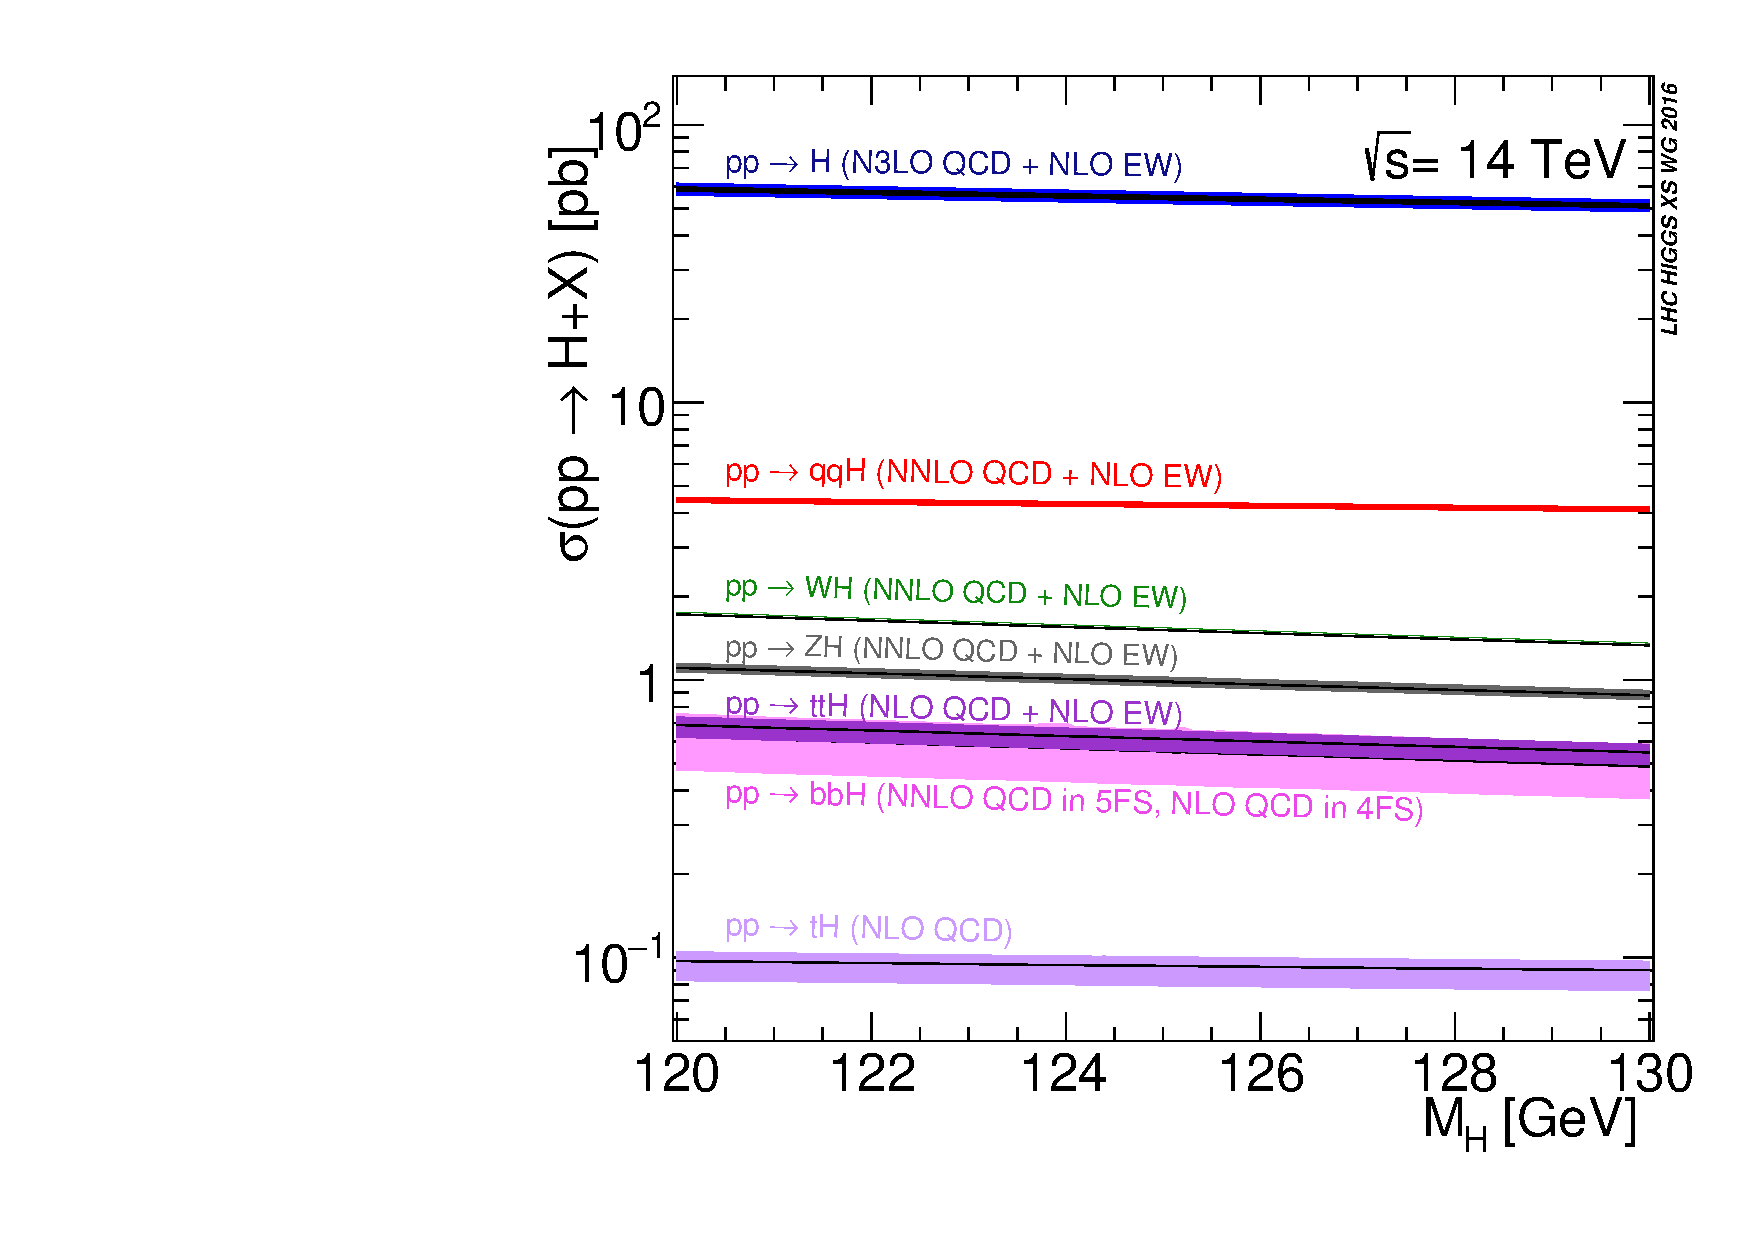
\includegraphics[scale=0.33]{H_cross_sections.pdf}}
\subfloat[][]{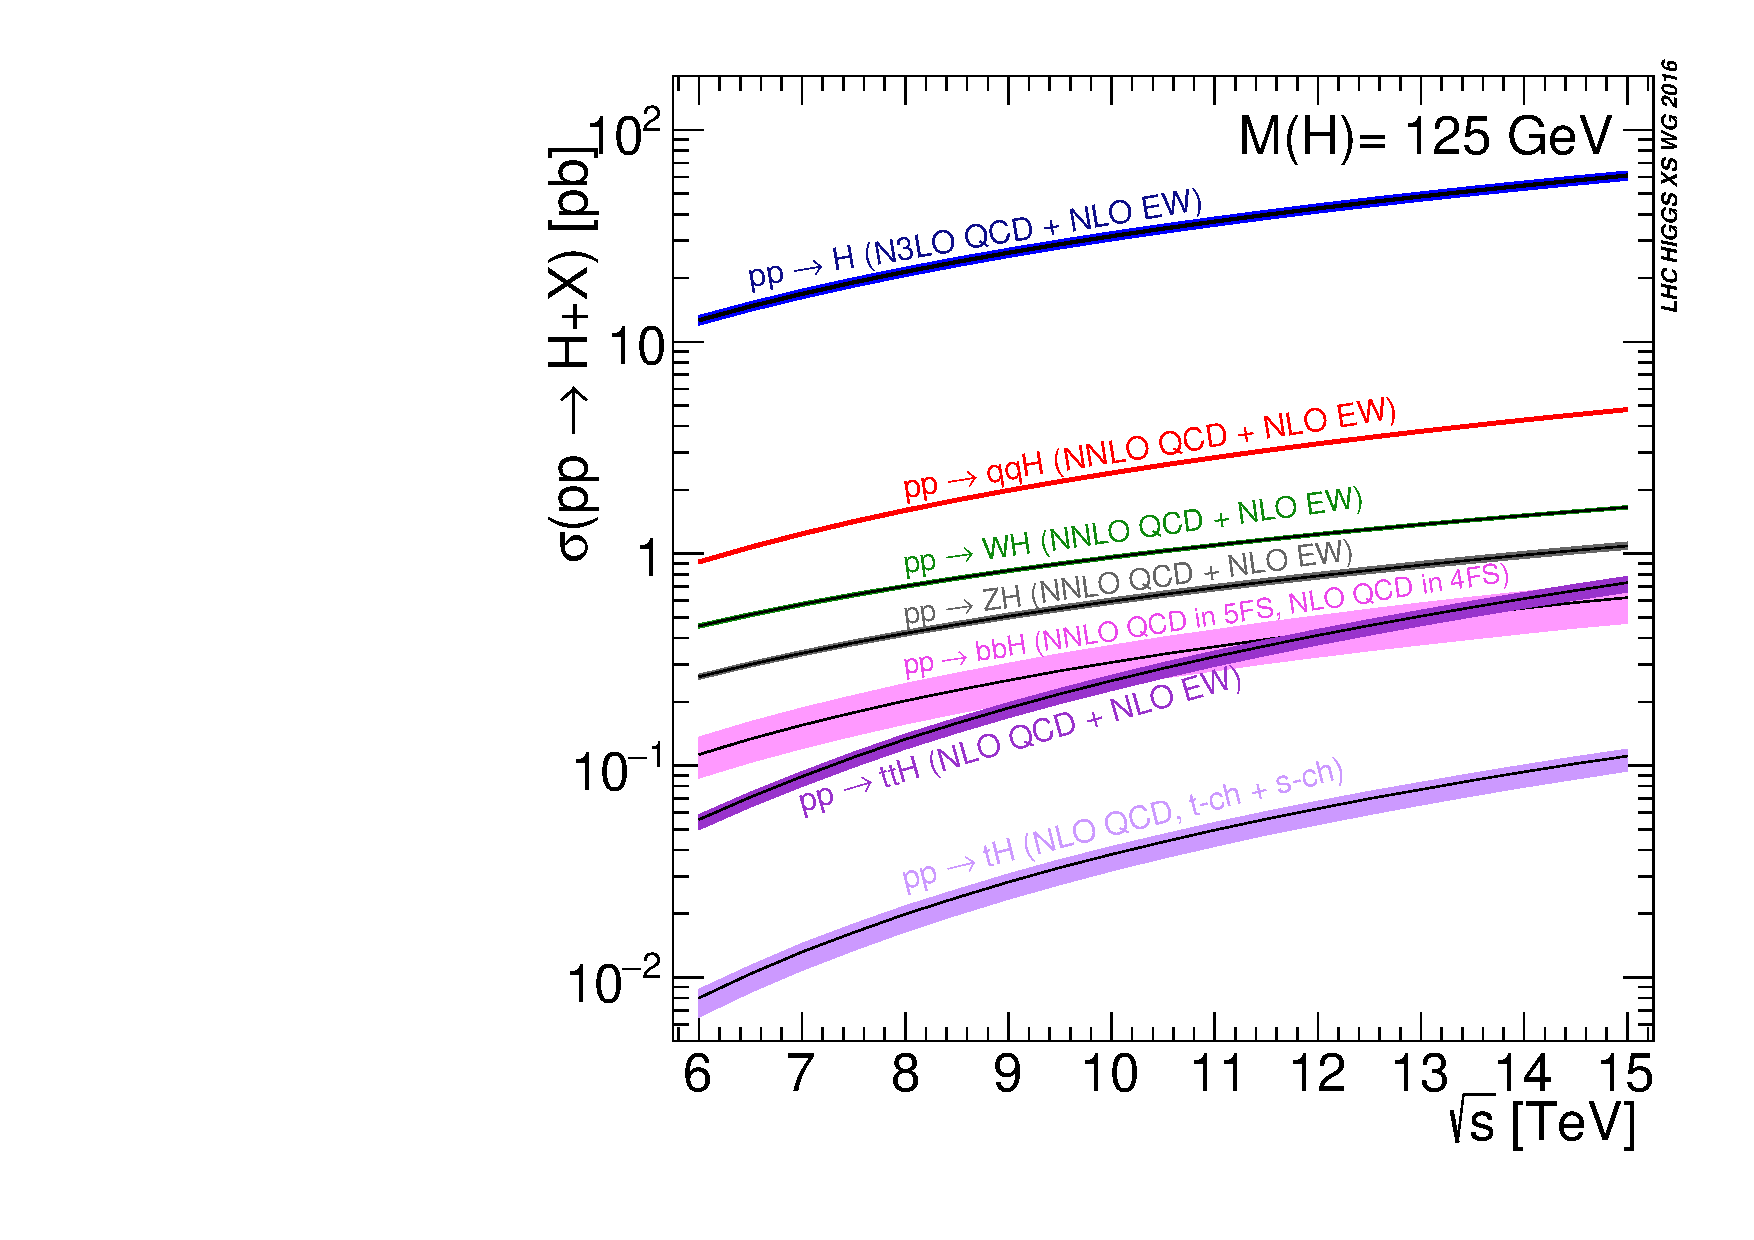
\includegraphics[scale=0.33]{cross_sec_energy.pdf}}
\caption{a)Higgs boson cross sections as a function of its mass for the various production modes, b)Higgs boson cross sections as a function of center-of-mass energy for the various production modes at $m_H = 125 \text{GeV}$.}
\label{H_cross_sections}
\end{figure}

\subsection{Higgs boson decay and the $\text{H} \rightarrow \gamma \gamma$ channel}
As any other Standard Model particle, the Higgs boson as well has a considerable manifold of processes concerning its decay channels. Each of these processes has a \emph{branching ratio} (BR), namely the fraction of decays that follows that process. These branching ratios are predicted by the Standard Model as a function of the Higgs mass (Figure \ref{H_BR}).
\\ \\
For very high masses, the leptonic decay channels mediated by W$^+$, W$^-$, or Z$^0$ bosons are the most probables for an Higgs event, while for masses up to around 130 GeV, the fermion-antifermion decay is the preferred decay mode and among the latter the $b\bar{b}$ stands out, because of its heavy mass and the consequent strong Higgs coupling.
\\
This large rate of $\text{gg} \rightarrow \text{H} \rightarrow \text{b}\bar{\text{b}}$ processes, on the other hand, has to compete with a very large background arising from the inclusive $\text{pp} \rightarrow \text{b}\bar{\text{b}} + \text{X}$due to the strong interaction.
\\
More simple to investigate becomes in this way the $\text{gg} \rightarrow \text{H} \rightarrow \gamma\gamma$ channel, where the Higgs boson decay into a pair of photons through a boson-loop or a fermion-loop, usually the W bosons are the most involved into the loop because of their strong coupling with the Higgs boson.
\begin{figure*}[h]
\centering
\subfloat{
	\feynmandiagram [small, horizontal=t1 to g1] {
  g1 --[boson] t1 -- [fermion] t2 --[fermion] t3 --[fermion] t1,
  g2 --[boson] t2,
  h -- [scalar, edge label = \small$H$]  t3,
  g1 --[opacity=0] g2,
};} \qquad
\subfloat{
	\feynmandiagram [small, horizontal=t1 to g1] {
  g1 --[boson] t1 -- [boson] t2 --[boson] t3 --[boson] t1,
  g2 --[boson] t2,
  h -- [scalar, edge label = \small$H$]  t3,
  g1 --[opacity=0] g2,
};}
\end{figure*}
\\The background for this channel derive from the processes with $\gamma\gamma$ and $\gamma$ + jet/dijet final states and can be splitted into two different categories: the reducible and the irreducible background. 
\\
\begin{itemize}
\item The reducible background is typically due to a $\pi^0$ decay from a main vertex of the hadronization jet. This kind of background it's quite easy to recognise, because the jet's deriving $\gamma$s not pass the photon isolation requirement for an Higgs event.
\item The irreducible background is composed of events where two photons are produced isolated, as well as for the signal. Typically the photons from these processes are produced directly in the main vertex and not in the jets, so they are isolated like the signal for the Higgs and it is not possible to distinguish between the two different kinds of events \cite{mass_measurement_ATLAS}.
\end{itemize}
\begin{figure}[htb]
\centering
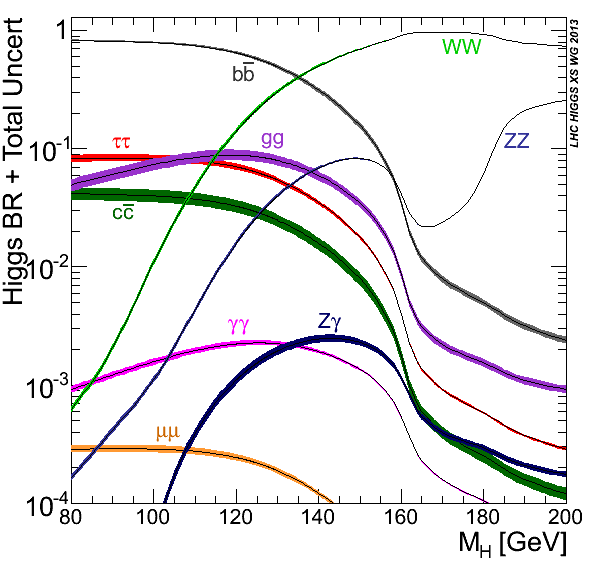
\includegraphics[scale=0.3]{H_BR.png}
\caption{Branching ratios for all of the Higgs decays, running over the whole mass spectrum.}
\label{H_BR}
\end{figure} 

\subsection{Experimental Higgs boson highlights}
Immediately after the discovery made by the ATLAS and CMS collaboration\cite{Observation_Higgs}, a considerable amount of measurements of the Higgs boson features has been performed, in order to establish the properties of the particle. Even if studies for such exotic beyond Standard Model Higgs bosons multiplets are still running, latest results from both the experiments involved in the research are consistent with Standard Model expectations for the Higgs boson.
\\\\
Starting from the mass measurement, achieved using Run1 results for $\text{H} \rightarrow \text{ZZ}^*$ and $\text{H} \rightarrow \gamma\gamma$ processes of both ATLAS and CMS experiments, which is found to be $m_H = 125.09 \pm 0.24 (\text{stat.}) \pm 0.11 (\text{syst.}) \text{GeV}$\cite{Aad2015zhl}, many other properties are still under investigation:
\begin{itemize}
\item the signal strength modifier $\mu$,
\item the couplings with fermions and bosons and their relative coupling-strength modifiers $k_j$,
\item the total decay width of the resonance of the particle
\end{itemize}
The signal strength $\mu_i$, which is the ratio between the observed production cross section $\sigma_i$ and the Standard Model's predicted value $\sigma_{SM}$ for a given mass hypothesis
\begin{equation}
\mu_i = \frac{\sigma_i}{\sigma_i^\text{SM}} \hspace{1cm} i \hspace{0.1cm} \text{: production modes}
\end{equation}
has been measured for each production mode separately.
\phantom{i}
\\
\phantom{i}
\begin{figure}[htb]
\centering
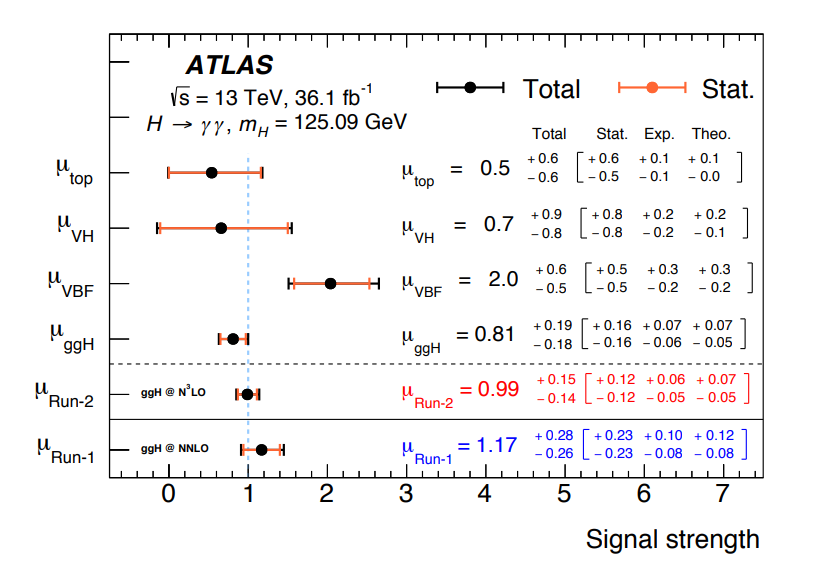
\includegraphics[scale=0.3]{signal_strength.png}
\caption{Signal strength's values measured for the different production modes (ggH, VBF, VH and top) and globally ($\mu_{Run2}$), compared with the global value ($\mu_{Run1}$).}
\end{figure}
\\The best-fit value for the signal strength, calculated for each production mode and corresponding to the measured mass of the particle, is found to be 
\begin{equation}
\mu_{ggH} = 0.81\hspace{0.06cm}^{+0.19}_{-0.18}\hspace{0.2cm} \text{,} \hspace{0.4cm} \mu_{VBf} = 2.0\hspace{0.06cm}^{+0.6}_{-0.5} \hspace{0.2cm} \text{,} \hspace{0.4cm} \mu_{VH} = 0.7\hspace{0.06cm}^{+0.9}_{-0.8} \hspace{0.2cm} \text{,} \hspace{0.4cm} \mu_{top} = 0.5\hspace{0.06cm}^{+0.6}_{-0.6} \hspace{0.4cm} \text{.}
\end{equation}
Then, the combination of all of the production modes brings to a value for the combined signal strength of
\begin{equation}
\mu_{comb} = 0.99\hspace{0.06cm}^{+0.15}_{-0.14}
\end{equation}
As well as the signal strength is the ratio between observed and predicted cross section, the coupling strength $k_i^2$ is the ratio between the observed coupling of the considered process $g_i$ and its predicted value for that process $g_i^{SM}$.
\begin{figure}[!b]
\centering
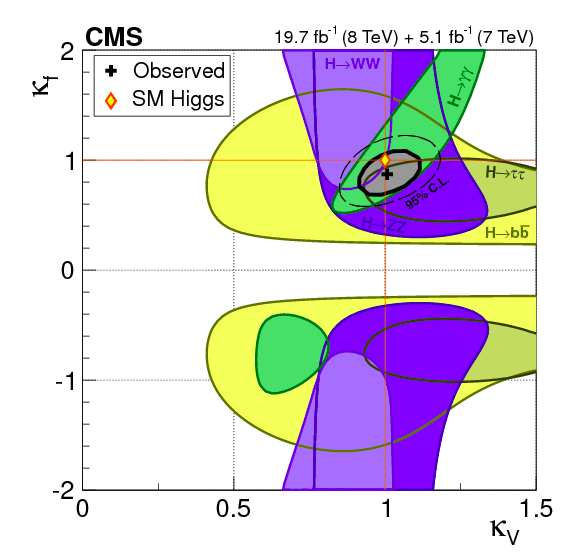
\includegraphics[scale=0.37]{kb_kv_Higgs.png}
\caption{Measurements of universal couplings for each production mode. The Model confirms the Standard Model prediction at 68\% CL.}
\end{figure}
\\In the k-framework, the cross section for an entire Higgs process is
\begin{equation}
\sigma(i \rightarrow H \rightarrow f) = \frac{\sigma_i(\vec{k}) \cdot \Gamma^f(\vec{k})}{\Gamma_H} \hspace{0.6cm}
\end{equation}
and all the possible deviations from the Standard Model predictions are described by the $k_j$ functions trough the relation
\begin{figure}[htb]
\centering
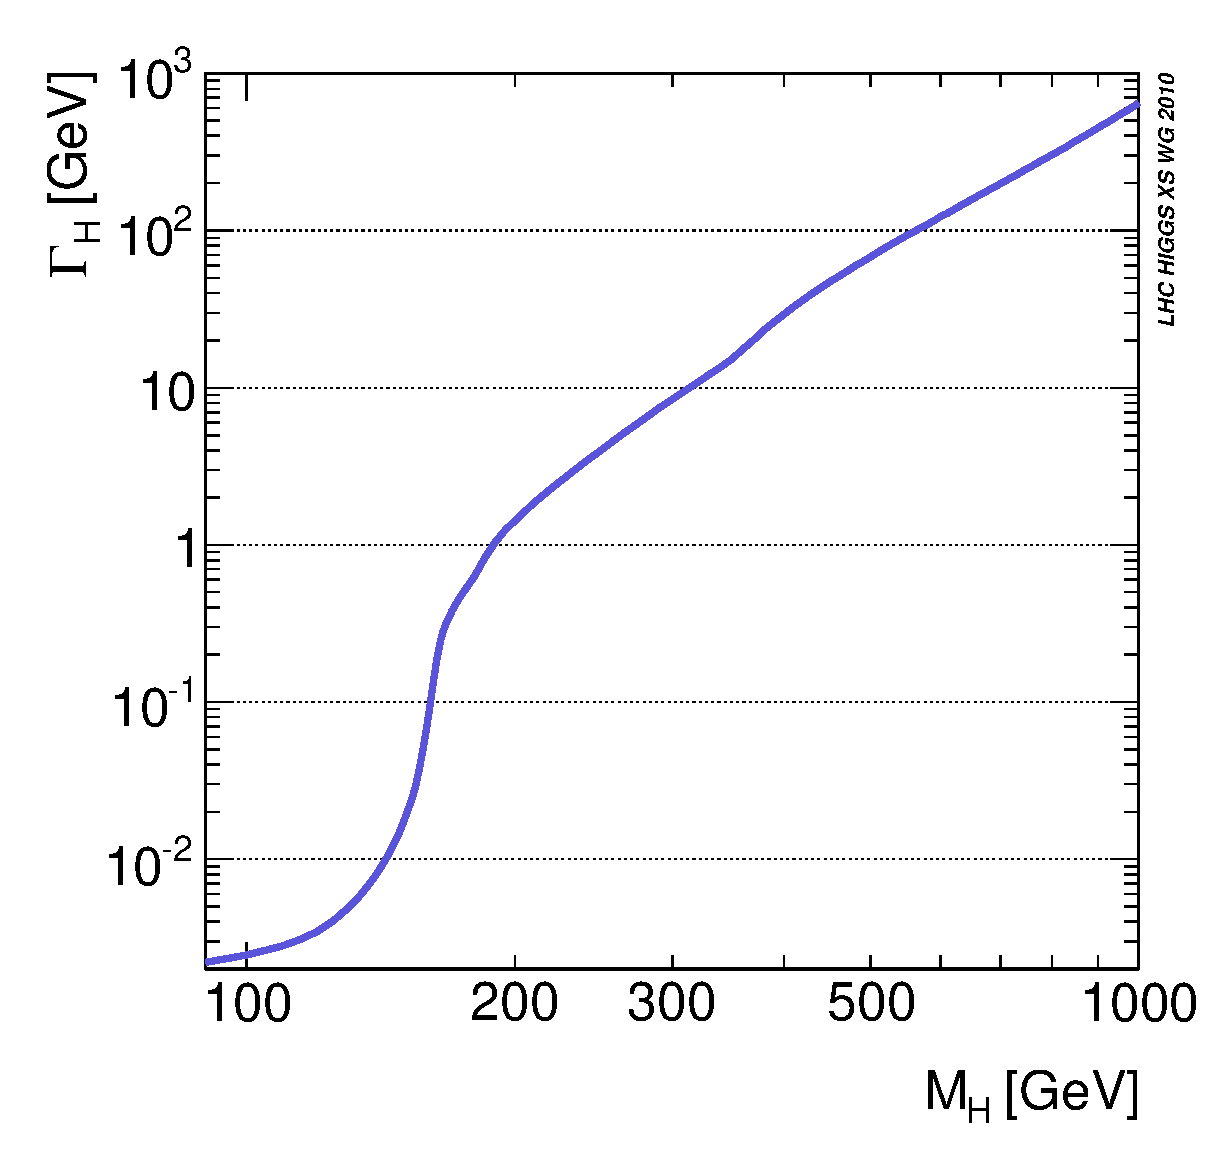
\includegraphics[scale=0.36]{total_decay_rate_Higgs.eps}
\caption{Total decay width for the Higgs boson predicted by Standard Model, as a function of it mass $m_H$.}
\label{total_decay_rate}
\end{figure}
\phantom{i}
\begin{equation}
\sigma_i = k_i^2(\vec{k}) \cdot \sigma_i^{\text{SM}} \hspace{0.4cm} \Longrightarrow \hspace{0.4cm} \Gamma^f = k_f^2(\vec{k}) \cdot \Gamma^{f, \text{SM}}
\end{equation}
Can be assured a universal coupling modifier $k_F$ for all fermions, and similarly a universal coupling modifier $k_V$ for all vector bosons.
\\
The total decay rate in the Standard Model is predicted as a function of the Higgs mass. In Figure \ref{total_decay_rate} you can see how, for masses of $m_H \simeq 125 \text{GeV}$, the total width is predicted by the Standard Model as a narrow resonance, with a total decay width of around 4.1 MeV. Combining results from different decays, the upper limit at 95\% CL on Higgs boson total decay width is calculated to be \cite{Khachatryan2016}
\begin{equation}
\Gamma_H^{\text{obs}} < 13 \text{MeV} \hspace{0.2cm} \text{.}
\end{equation}